\documentclass[aspectratio=169]{beamer}

% Document metadata
\title{Conceitos Básicos de Git e GitHub}
\subtitle{Material para servir de apoio e revisão}
\author[E. Goto]{Erik Goto}
\institute{UNICAMP}
\date{\today}

% Image for the title page (use includegraphics option to properly size/place it)
%\titlegraphic{
\includegraphics[height=\paperheight]{library.jpg}}

\usetheme[sectionstyle=style2]{trigon}

% Define logos to use (comment if no logo)
\biglogo{git.png} % Used on titlepage only
%\smalllogo{git.png} % Used on top right corner of regular frames

% ------ If you want to change the theme default colors, do it here ------
%\definecolor{tPrim}{HTML}{00843B}   % Green
%\definecolor{tSec}{HTML}{289B38}    % Green light
\definecolor{tAccent}{HTML}{F07F3C} % Orange


% ------ Packages and definitions used for this demo. Can be removed ------
\usepackage{appendixnumberbeamer} % To use \appendix command
\pdfstringdefDisableCommands{% Fix hyperref translate warning with \appendix
\def\translate#1{#1}%
}
\usepackage{pgf-pie} % For pie charts
\usepackage{caption} % For subfigures
\usepackage{subcaption} % For subfigures
\usepackage{xspace}
\newcommand{\themename}{\textbf{\textsc{trigon}}\xspace}
\usepackage[scale=2]{ccicons} % Icons for CC-BY-SA
\usepackage{booktabs} % Better tables
\usepackage[utf8]{inputenc}
\usepackage[brazilian]{babel}
\graphicspath{ {imagens/} }
\usepackage{multicol}
%==============================================================================
%                               BEGIN DOCUMENT
%==============================================================================
\begin{document}

%--------------------------------------
% Create title frame
\titleframe

%--------------------------------------
% Table of contents
\begin{frame}{Overview}
\setbeamertemplate{section in toc}[sections numbered]
	\begin{multicols}{3}
  \tableofcontents[hideallsubsections]
	\end{multicols}
  

\end{frame}
%==============================================
\section{Introduction}
%==============================================
\begin{frame}{\insertsectionhead}
  \framesubtitle{A short introduction to Trigon}
  \themename is a modern, elegant and versatile theme for Beamer, inspired by
  the
  \href{https://github.com/matze/mtheme}{\textsc{metropolis} theme} from Matthias
  Vogelgesang.
  \vfill
  \themename comes with lots of nice extra features
  \begin{itemize}
    \item Multiple style variations for title, section and normal slides
    \item Simple customization of theme colors
    \item Lots of convenient options to tweak the design
  \end{itemize}
\end{frame}


%==============================================
\section{Configurações}
%==============================================
\begin{frame}{\insertsectionhead}
	Configurações para identificar o computador, por meio do nome e endereço de email. Essas informações serão mostradas ao ver a autoria dos \textit{commits}
	\begin{block}{Nome}
		git config $--$global user.name \textit{seu nome}
	\end{block}
	\begin{block}{Email}
		git config $--$global user.email \textit{email@gmail.com}
	\end{block}
	\begin{block}{Visualizar as configurações}
		git config $--$list
	\end{block}
\end{frame}

%==============================================
\section{Clone}
%==============================================
\begin{frame}{\insertsectionhead}
	Com o \textit{clone} é possível copiar um respositório do GitHub para uma pasta local do PC.\\
	Para tanto copie o link HTTPS, que pode ser encontrado na página do projeto:
	\begin{figure}
		\centering
		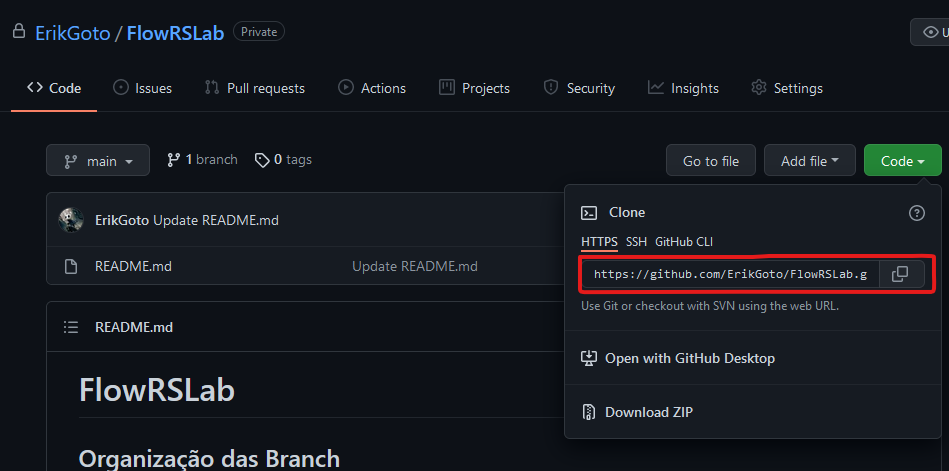
\includegraphics[scale=0.4]{a.png}
		\caption{Clone}
	\end{figure}
	
\end{frame}
\begin{frame}
	Com o \textit{git bash} escolha a pasta de destino no computador, e execute o \textit{clone}
	\begin{block}{Clone}
		git clone https://github.com/ErikGoto/FlowRSLab.git
	\end{block}
	\begin{figure}
		\centering
		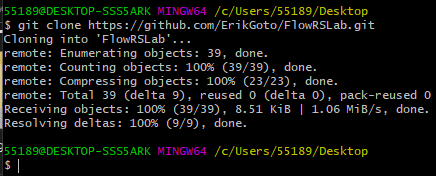
\includegraphics[scale=0.6]{aa.png}
		\caption{Git Bash - Clone}
	\end{figure}
\end{frame}

%==============================================
\section{Salvando Alterações}
%==============================================
\begin{frame}{\insertsectionhead}
	De maneira \textit{super simplificada}, para salvar as alterações realizadas basta usar dois comandos dentro da pasta onde o git foi inicializado:
	\begin{block}{Add}
		git add .
	\end{block}
	\begin{block}{Commit}
		git commit -m "Mensagem de commit"
	\end{block}
	A \textit{mensagem de commit} precisa ser um texto explicativo sobre as alterações, e referente ao commit realizado. 
	
\end{frame}

%==============================================
\section{Histórico de Commit - Log}
%==============================================
\begin{frame}{\insertsectionhead}
	Para visualizar o histórico de commit usamos o comando log
	\begin{block}{Log}
		git log $--$oneline
	\end{block}
	
\end{frame}

%==============================================
\section{Ramificações - Branch}
%==============================================
\begin{frame}{\insertsectionhead}
	\begin{block}{Segundo o Atlassian\footnote{\url{https://www.atlassian.com/br/git/tutorials/using-branches}}, a definição de uma branch}
		Quando você quiser adicionar um novo recurso ou corrigir um bug—não importa o tamanho, grande ou pequeno—basta criar uma nova ramificação para encapsular as mudanças. Isso faz com que seja mais difícil um código instável ser mesclado com a base de código principal e dá a chance de você limpar seu histórico futuro antes de fazer a mesclagem na ramificação principal.
	\end{block}
\end{frame}
\begin{frame}
	Para criar uma ramificação nova (ou branch) e mudar para a mesma, usamos dois comandos:
	\begin{block}{Criar}
		git branch nova\_ branch
	\end{block}
	\begin{block}{Mudar para a branch}
		git checkout nova\_ branch
	\end{block}
	Ou de forma simplificada:
	\begin{block}{Realiza os dois passos anteriores de uma única vez}
		git checkout -b nova\_ branch
	\end{block}
\end{frame}
\begin{frame}
	\begin{figure}
		\centering
		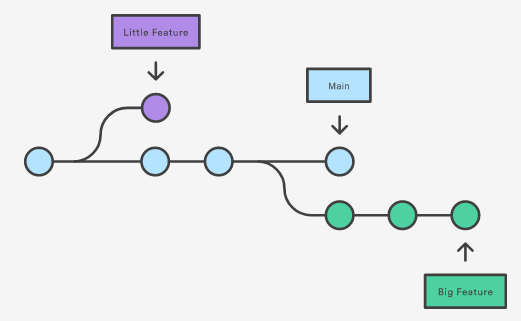
\includegraphics[scale=0.8]{aaa.png}
		\caption{Branch}
	\end{figure}
\end{frame}
\begin{frame}
	Outros comandos úteis:
	\begin{block}{Visualizar todas as branches}
		git branch
	\end{block}
	\begin{block}{Deleta uma branch específica}
		git -d \textit{nome\_ branch}
	\end{block}
\end{frame}

%==============================================
\section{Voltando para versões anteriores}
%==============================================
\begin{frame}{\insertsectionhead}

\end{frame}

%==============================================
\section{Interações com o GitHub - Pull e Push}
%==============================================
\begin{frame}{\insertsectionhead}
	O comando \textit{pull} serve para "puxar" \ os arquivos da nuvem para o repositório local.\\
	Enquanto o comando \textit{push} "empurra" \ do repositório local para a nuvem.
	\begin{block}{Pull}
		git pull origin nome\_ branch
\end{block}	 
	\begin{block}{Push}
		git push origin nome\_ branch
	\end{block}
\end{frame}
\begin{frame}
	Quando damos um push de uma branch para o GitHub aparece a opção de um pull request na página do projeto:
	\begin{figure}
		\centering
		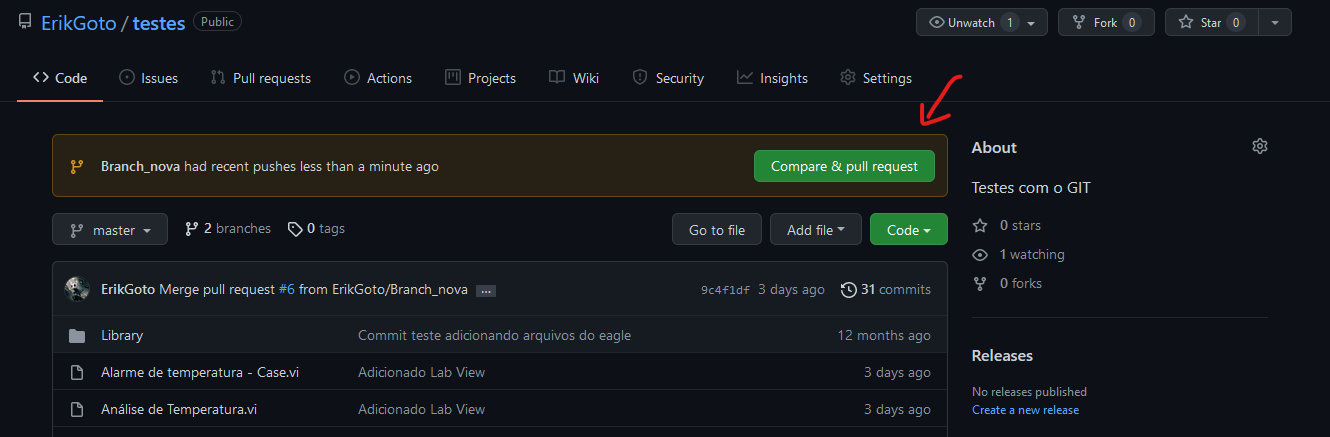
\includegraphics[scale=0.4]{a1.png}
		\caption{Clone}
	\end{figure}
\end{frame}
\begin{frame}
	Clique para criar uma pull request. Você será direcionado para a seguinte página
	\begin{figure}
		\centering
		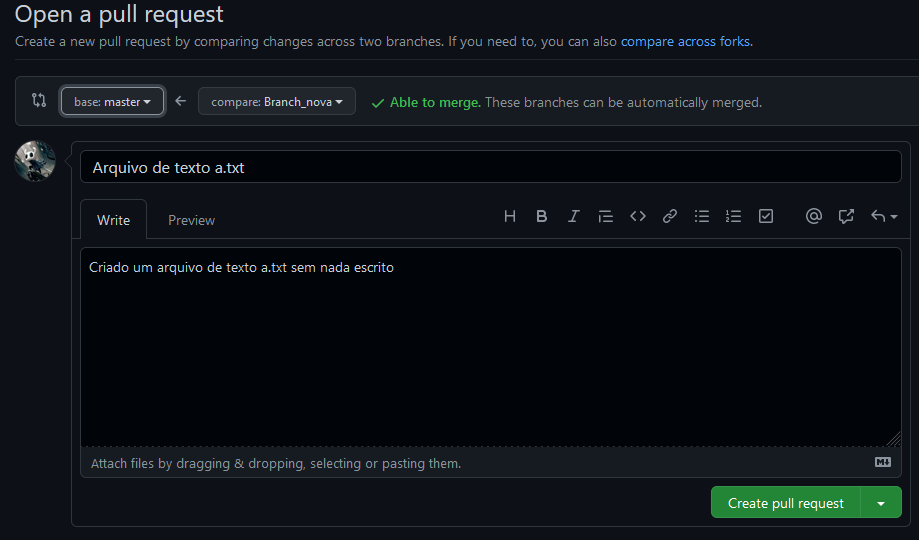
\includegraphics[scale=0.4]{a2.png}
		\caption{Clone}
	\end{figure}
	Aqui é possível definir um título, descrição e \textit{selecionar a branch} onde ocorrerá o \textit{merge}
\end{frame}
\begin{frame}
	\frametitle{Selecionando a branch para o merge}
	\begin{figure}
		\centering
		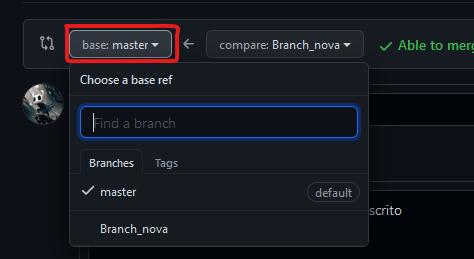
\includegraphics[scale=0.8]{a3.png}
		\caption{Clone}
	\end{figure}
\end{frame}
\begin{frame}
	Após isso, basta clicar em \textit{Create Pull Request}.
	Depois que as alterações da branch forem revisadas clique em \textit{Merge Pull request} para dar um merge à branch escolhida, e delete a branch do pull request.
	\begin{figure}
		\centering
		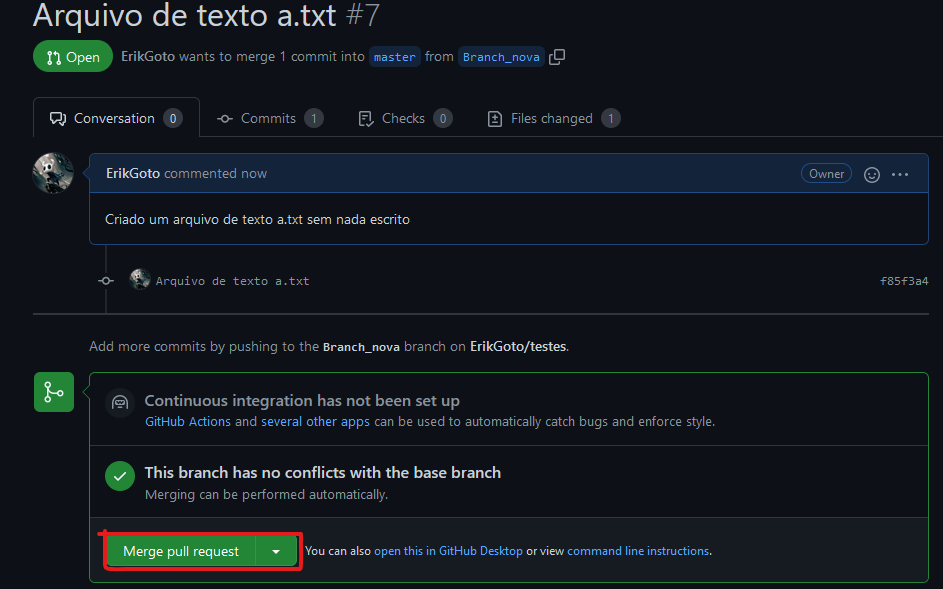
\includegraphics[scale=0.4]{a4.png}
		\caption{Clone}
	\end{figure}
\end{frame}
%==============================================
\section{Tags e Releases}
%==============================================
\begin{frame}{Tags}
	\begin{block}{Cria Tag}
		git tag -a v0.1 -m "Nome da Tag"
	\end{block}
	\begin{block}{Lista todas as tags}
		git tag
	\end{block}
	\begin{block}{Envia a tag para o GitHub}
		git push --tag
	\end{block}
	
	
	
	
\end{frame}
\begin{frame}{Release}
	\begin{figure}
		\centering
		
\includegraphics[scale=0.4]{a5.png}
		\caption{Clone}
	\end{figure}
\end{frame}
\begin{frame}
	\begin{figure}
		\centering
		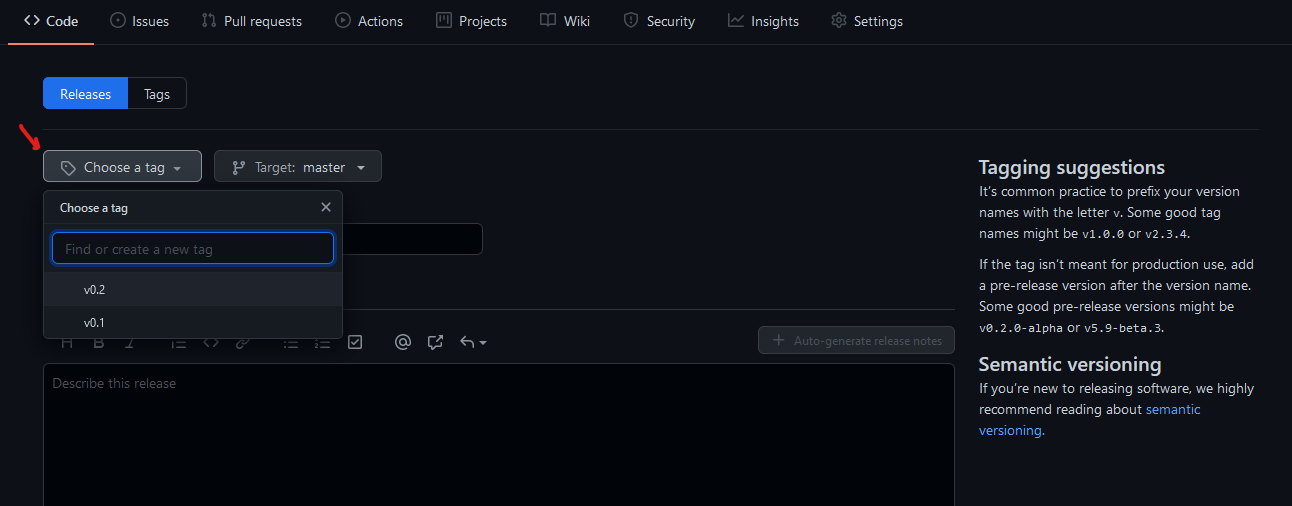
\includegraphics[scale=0.4]{a6.png}
		\caption{Clone}
	\end{figure}
\end{frame}
\begin{frame}
	\begin{figure}
		\centering
		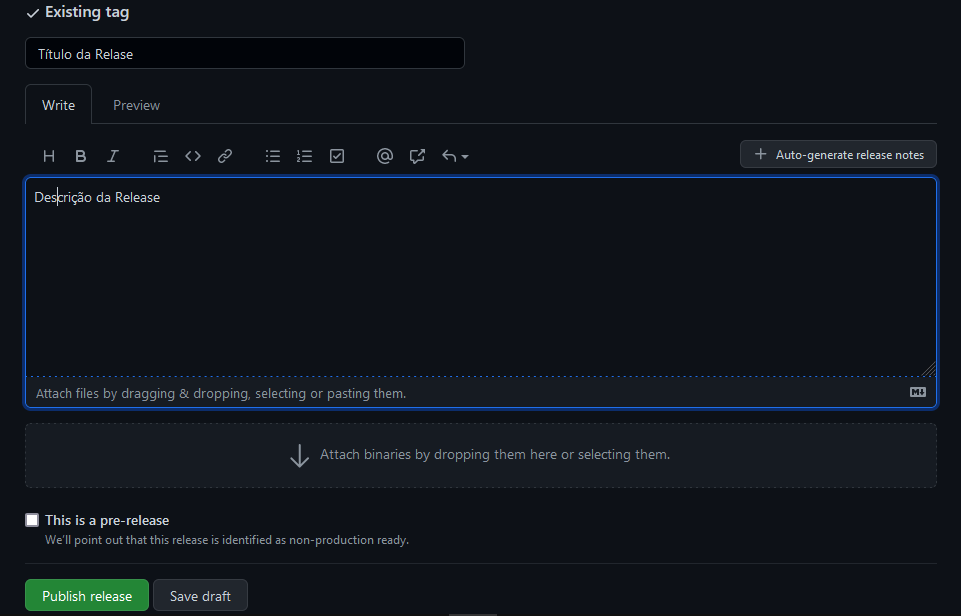
\includegraphics[scale=0.4]{a7.png}
		\caption{Clone}
	\end{figure}
\end{frame}
\begin{frame}
	\begin{figure}
		\centering
		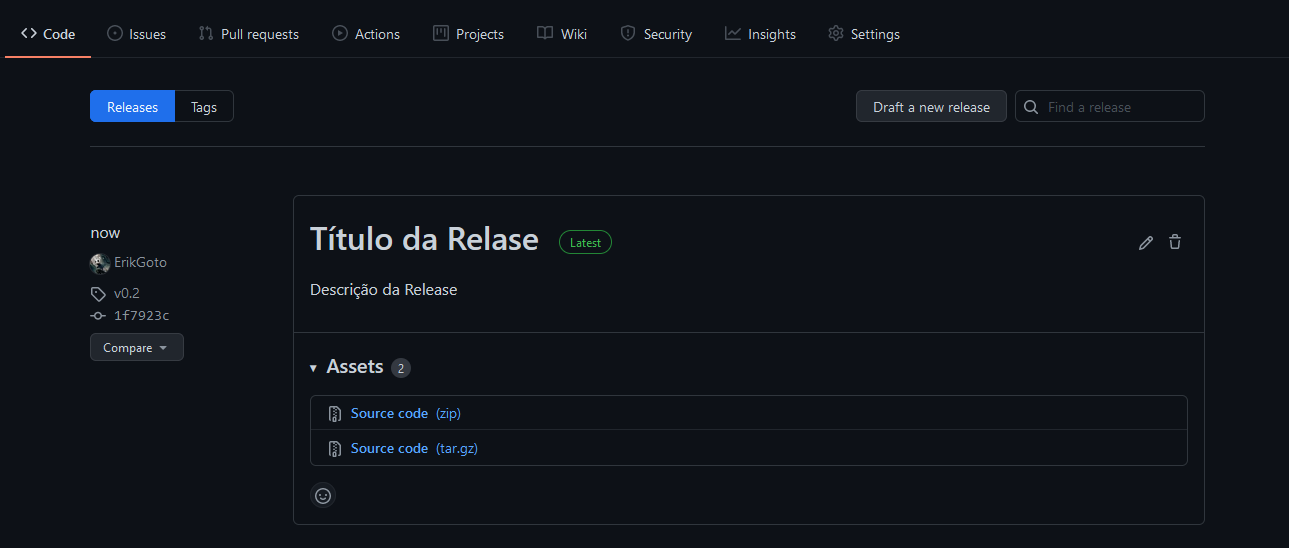
\includegraphics[scale=0.4]{a8.png}
		\caption{Clone}
	\end{figure}
\end{frame}

%==============================================
\section{Fontes}
%==============================================
\begin{frame}
	\begin{itemize}
		\item Template da Apresentação: Thomas Lambert - \url{https://pt.overleaf.com/latex/templates/trigon-beamer-theme/wjyyzvdzqkgf}
		\item Git e GitHub para iniciantes – Tutorial completo - \url{https://fullcycle.com.br/git-e-github/}
		\item Git Branch - \url{https://www.atlassian.com/br/git/tutorials/using-branches}
	\end{itemize}
	\end{frame}

\end{document}
